\documentclass[12pt]{article}
\usepackage[margin=1in]{geometry}
\usepackage[all]{xy}


\usepackage{amsmath,amsthm,amssymb,color,latexsym}
\usepackage{geometry}        
\geometry{letterpaper}    
\usepackage{graphicx}

\usepackage{listings}
\usepackage{xcolor}

\usepackage[export]{adjustbox}

\definecolor{codegreen}{rgb}{0,0.6,0}
\definecolor{codegray}{rgb}{0.5,0.5,0.5}
\definecolor{codepurple}{rgb}{0.58,0,0.82}
\definecolor{backcolour}{rgb}{0.95,0.95,0.92}

\lstdefinestyle{mystyle}{
  backgroundcolor=\color{backcolour},   commentstyle=\color{codegreen},
  keywordstyle=\color{magenta},
  numberstyle=\tiny\color{codegray},
  stringstyle=\color{codepurple},
  basicstyle=\ttfamily\footnotesize,
  breakatwhitespace=false,         
  breaklines=true,                 
  captionpos=b,                    
  keepspaces=true,                 
  numbers=left,                    
  numbersep=5pt,                  
  showspaces=false,                
  showstringspaces=false,
  showtabs=false,                  
  tabsize=2
}

\lstset{style=mystyle}

\usepackage{graphicx}
\graphicspath{ {./images/} }


\newtheorem{problem}{Problem}

\newenvironment{solution}[1][\it{Solution}]{\textbf{#1. } }{$\square$}


\begin{document}
\noindent CS 6140: Machine Learning Spring 2021\hfill Homework Assignment \#1\\
Sai Nikhil (02/06/2021)\hfill thirandas.s@northeastern.edu

\hrulefill


\begin{problem}
Let $X, Y$ and $Z$ be discrete random variables defined as functions on the same probability space $(\Omega, \mathcal{A}, P) .$ Prove or disprove the following expression
$$
P(X=x \mid Y=y)=\sum_{z \in \mathcal{Z}} P(X=x \mid Y=y, Z=z) \cdot P(Z=z \mid Y=y)
$$
where $\mathcal{Z}$ is the sample space defined by the random variable $Z$.
\end{problem}
\begin{solution}
We know that,
\begin{align*}
P(X=x, Y=y, Z=z)=P(Y=y) \cdot P(Z=z \mid Y=y) \cdot P(X=x \mid Z=z, Y=y)
\end{align*}
Therefore,
\begin{align*}
\sum_{z \in \mathcal{Z}} P(X=x \mid Y=y, Z=z) \cdot P(Z=z \mid Y=y) & = \sum_{z \in \mathcal{Z}} \frac{P(X=x, Y=y, Z=z)}{P(Y=y)}\\
													& = \frac{P(X=x, Y=y)}{P(Y=y)} \\
													& = P(X=x \mid Y=y)
\end{align*}
\end{solution} 

\begin{problem}
Let $X$ be a random variable on $\mathcal{X}=\{a, b, c\}$ with the probability mass function $p(x) .$ Let $p(a)=0.1, p(b)=0.2,$ and $p(c)=0.7$ and some function $f(x)$ be
$$
f(x)=\left\{\begin{array}{ll}
10 & x=a \\
5 & x=b \\
\frac{10}{7} & x=c
\end{array}\right.
$$
a) (5 points) What is $\mathbb{E}[f(X)]$ ?\\
b) (5 points) What is $\mathbb{E}[1 / p(X)] ?$\\
c) (5 points) For an arbitrary finite set $\mathcal{X}$ with $n$ elements and arbitrary $p(x)$ on $\mathcal{X}$, what is $\mathbb{E}[1 / p(X)]$ ?
\end{problem}
\begin{solution}
$$
f(x)=\left\{\begin{array}{ll}
10 & x=a \\
5 & x=b \\
\frac{10}{7} & x=c
\end{array}\right.
$$
a)
\begin{align*}
\qquad \mathbb{E}[f(x)] & =\sum_{x \in \mathcal{X}} f(X=x) \times p(X=x) \\
& = 10 \times 0.1+5 \times 0.2+\frac{10}{7} \times 0.7 \\
& = \boxed{3}
\end{align*}
b)
\begin{align*}
\mathbb{E}\left[\frac{1}{p(X)}\right] &=\sum_{x \in \mathcal{X}} \frac{1}{p(X=x)} \times p(X = x) \\
&=1+1+1 \\
&=\boxed{3}
\end{align*}
c)
Let, 
$$
\mathcal{X} = \left\{x_{1}, x_{2}, \ldots, x_{n}\right\}
$$
\begin{align*}
\mathbb{E}\left[\frac{1}{p(x)}\right] &=\sum_{x \in \mathcal{X}} \frac{1}{p(X=x)} \times p(X=x) \\
&=\sum_{i=1}^{n} 1 \\
&=\boxed{n}
\end{align*}
\end{solution}


\begin{problem}
A biased four-sided die is rolled and the down face is a random variable $X$ described by the following $\mathrm{pmf}$
$$
p(x)=\left\{\begin{array}{ll}
x / 10 & x=1,2,3,4 \\
0 & \text { otherwise }
\end{array}\right.
$$
Given the random variable $X$ a biased coin is flipped and the random variable $Y$ is 1 or zero according to whether the coin shows heads or tails. The conditional pmf is
$$
p(y \mid x)=\left(\frac{x+1}{2 x}\right)^{y}\left(1-\frac{x+1}{2 x}\right)^{1-y}
$$
where $y \in\{0,1\}$.\\
a) (5 points) Find the expectation $\mathbb{E}[X]$ and variance $V[X]$.\\
b) (5 points) Find the conditional $\operatorname{pmf} p(x \mid y)$.\\
c) (5 points) Find the conditional expectation $\mathbb{E}[X \mid Y=1] ;$ i.e., the expectation with respect to the conditional $\operatorname{pmf} p_{X \mid Y}(x \mid 1)$.
\end{problem}

\begin{solution}
Given,
$$
p(x)=\left\{\begin{array}{ll}
x / 10 & x=1,2,3,4 \\
0 & \text { otherwise }
\end{array}\right.
$$
$$
p(y \mid x)=\left(\frac{x+1}{2 x}\right)^{y}\left(1-\frac{x+1}{2 x}\right)^{1-y}
$$
where $y \in\{0,1\}$.\\
a)
\begin{align*}
\mathbb{E}[x] &=\sum_{x \in\{1,2,3,4\}} x \cdot p(X=x) \\
&=1 \times \frac{1}{10}+2 \times \frac{2}{10}+3 \times \frac{3}{10}+4 \times \frac{4}{10} \\
&=\frac{30}{10}\\
&=\boxed{3}\\\\
\mathbb{E}\left[X^{2}\right] &=\sum_{x \in \mathcal{X}} x^{2} p(X=x) \\
&=1^{2} \times \frac{1}{10}+2^{2} \times \frac{2}{10}+3^{2} \times \frac{3}{10}+4^{2}\times\frac{4}{10}\\
&=10\\\\
\mathbb{V}\left[X\right] &= \mathbb{E}\left[X^{2}\right] - \left(\mathbb{E}\left[X\right]\right)^{2}\\
&= 10 - 9\\
&= \boxed{1}
\end{align*}
b)
\begin{align*}
p(x \mid y)&=\frac{p(y \mid x) p(x)}{p(y)}\\
&=\frac{p(y \mid x) \times p(x)}{\sum_{x \in \mathcal{X}} p(y \mid x) \times p(x)}\\
&=\frac{\left(\frac{x+1}{2 x}\right)^{y}\left(1-\frac{x+1}{2 x}\right)^{1-y} \times \frac{x}{10}}{\left({\frac{2}{2}}^{y} \times 0^{1-y} \times \frac{1}{10}+\left(\frac{3}{4}\right)^{y}\left(\frac{1}{4}\right)^{1-y}\times\frac{2}{10}+\left(\frac{2}{3}\right)^{y}\left(\frac{1}{3}\right)^{1-y}\times\frac{3}{10}+\left(\frac{5}{8}\right)^{y}\left(\frac{3}{8}\right)^{1-y}\times\frac{4}{10}\right)}\\
&=\frac{2 \times \left(\frac{x+1}{2 x}\right)^{y}\left(1-\frac{x+1}{2 x}\right)^{1-y} \times x}{\left(1^{y} \times 0^{1-y} \times 2+3^{y}\times1^{1-y}\times4+4^{y}\times2^{1-y}\times6+5^{y}\times3^{1-y}\times8\right)}\\
\end{align*}
Writing it in piecewise form,
$$
p(x \mid y)=\left\{\begin{array}{ll}
\frac{x-1}{6} & y=0 \\
\frac{x+1}{14} & y=1
\end{array}\right.
$$

c)
\begin{align*}
\mathbb{E}[X \mid Y=1]=\sum_{x \in \mathcal{X}} x \cdot p_{X \mid Y}(x \mid 1)
\end{align*}

\begin{align*}
p_{X \mid Y}(x \mid 1)&=\frac{\left(\frac{x+1}{2x}\right)^{1} \times\left(1-\frac{x+1}{2 x}\right)^{0} \times \frac{x}{10}}{1^{1} \times 0^{0} \times \frac{1}{10}+\left(\frac{3}{4}\right)^{1} \times\left(\frac{1}{4}\right)^{0} \times \frac{2}{10} + \left(\frac{4}{6}\right)^{1} \times\left(\frac{2}{6}\right)^{0} \times \frac{3}{10} + \left(\frac{5}{8}\right)^{1} \times\left(\frac{3}{8}\right)^{0} \times \frac{4}{10}}\\
&=\frac{x+1}{14}
\end{align*}

\begin{align*}
\mathbb{E}[X \mid Y=1] &= \sum_{x \in \mathcal{X}} x \times \frac{x + 1}{14}\\
&= 1 \times \frac{2}{14} + 2 \times \frac{3}{14} + 3 \times \frac{4}{14} + 4 \times \frac{5}{14}\\
&= \boxed{\frac{20}{7}} 
\end{align*}

\end{solution}



\begin{problem}
Suppose that the data set $\mathcal{D}=\{1,0,1,1,1,0,1,1,1,0\}$ is an i.i.d. sample form a Bernoulli distribution
$$
p(x \mid \alpha)=\alpha^{x}(1-\alpha)^{1-x} \quad 0<\alpha<1
$$
with an unknown parameter $\alpha$.\\
a) (5 points) Calculate the log-likelihood of the data $\mathcal{D}$ when $\alpha=\frac{1}{e} ;$ i.e., find $\log p(\mathcal{D} \mid \alpha=\frac{1}{e})$. The parameter $e$ is the Euler number. Write the final expression as compactly as you can.\\
b) (10 points) Compute the maximum likelihood estimate of $\alpha$. Show all your work.\\
c) (10 points) Suppose the prior distribution for $\alpha$ is the uniform distribution on (0,1).  Compute the Bayes estimator for $\alpha .$ Note that $\int_{0}^{1} v^{m}(1-v)^{r} d v=\frac{m ! r !}{(m+r+1) !}$
\end{problem}

\begin{solution}
a)
\begin{align*}
p(\mathcal{D} \mid \alpha) &= p(\left\{x_i\right\}_{i=1}^{n} \mid \alpha)\\
&= \prod_{i=1}^{n} p(x_i \mid \alpha)\\
&= \alpha^{\sum_{i=1}^{n}x_i} \cdot \left(1-\alpha \right)^{n - \sum_{i=1}^{n}x_i}\\
\end{align*}

\begin{align*}
ll\left(\mathcal{D}, \alpha\right) &= \ln \alpha \cdot \sum_{i=1}^{n}x_i + \ln \left(1-\alpha \right) \cdot \left(n-\sum_{i=1}^{n}x_i\right)\\
ll\left(\mathcal{D}, \frac{1}{e}\right) &= 3\ln\left(e-1\right)-10
\end{align*}

b)
\begin{align*}
\frac{\partial ll\left(\mathcal{D}, \alpha\right)}{\partial \alpha} &= \frac{\sum_{i=1}^{n}x_i}{\alpha} - \frac{n-\sum_{i=1}^{n}x_i}{1-\alpha}\\
&=0
\end{align*}
\begin{align*}
\implies \left(1-\alpha_{ML} \right) \cdot \sum_{i=1}^{n}x_i - \left(n - \sum_{i=1}^{n} x_i \right) \cdot \alpha_{ML} = 0\\
\alpha_{ML} = \frac{\sum_{i=1}^{n}x_i}{n} = \boxed {\frac{7}{10}}
\end{align*}

c)
\begin{align*}
p\left(\mathcal{D}\mid\alpha\right) &= \alpha^{\sum_{i=1}^{n}x_i} \cdot (1-\alpha)^{n-\sum_{i=1}^{n}x_i}\\
p\left(\alpha\right) &= 1\\
p\left(\alpha \mid \mathcal{D}\right) &= \frac{p\left(\mathcal{D} \mid \alpha \right) \cdot p\left(\alpha\right)}{p\left( \mathcal{D} \right)}\\
p\left( \mathcal{D} \right) &= \int_{0}^{1} p\left(\mathcal{D} \mid \alpha \right) p\left(\alpha \right)\,d\alpha\\
&=\int_{0}^{1} \alpha^7 \left(1-\alpha\right)^3 \, d\alpha\\
&=\frac{7!\cdot3!}{11!}
\end{align*}

\begin{align*}
\alpha_{B} &= \int_{0}^{1} \alpha \, p\left(\alpha \mid \mathcal{D}\right) \, d\alpha\\
&= \int_{0}^{1}\frac{\alpha \times \alpha^7 \times \left(1-\alpha\right)^{3} \times 1}{p\left(\mathcal{D}\right)} \, d\alpha\\
&= \frac{\int_{0}^{1}\alpha^8 \times \left(1-\alpha \right)^{3} \, d\alpha}{\frac{7! \cdot 3!}{11!}}\\
&= \boxed{\frac{2}{3}}
\end{align*}
\end{solution}


\begin{problem}
Let $\mathcal{D}=\left\{x_{i}\right\}_{i=1}^{n}$ be an i.i.d. sample from
$$
p(x)=\left\{\begin{array}{ll}
e^{-\left(x-\theta_{0}\right)} & x \geq \theta_{0} \\
0 & \text { otherwise }
\end{array}\right.
$$
Determine $\theta_{\mathrm{ML}}$ - the maximum likelihood estimate of $\theta_{0}$.
\end{problem}
\begin{solution}

\begin{align*}
p(x)&=\left\{\begin{array}{ll}
e^{-\left(x-\theta_{0}\right)} & x \geq \theta_{0} \\
0 & \text { otherwise }
\end{array}\right.\\
\mathcal{D}&=\left\{x_{i}\right\}_{i=1}^{n}
\end{align*}

For $\theta_0 \le min\left(\left\{x_i\right\}_{i=1}^{n}\right)$, 
\begin{align*}
p\left(\mathcal{D} \mid \theta_0 \right) &= p\left(\left\{x_{i}\right\}_{i=1}^{n} \mid \theta_0\right)\\
&= \prod_{i=1}^{n}p\left(x_i \mid \theta_0\right)\\
&= e^{-\left(\sum_{i=1}^{n}x_i-n \cdot \theta_0\right)}
\end{align*}

For $\theta_0 > min\left(\left\{x_i\right\}_{i=1}^{n}\right)$, 
\begin{align*}
p\left(\mathcal{D} \mid \theta_0 \right) &= 0
\end{align*}

This is a strictly increasing function w.r.t.  $\theta_0$ until $\theta_0 = min\left(\left\{x_i\right\}_{i=1}^{n}\right)$ and then falls to $0$ after that.\\

Thefore, the maximum likelihood

$$\theta_{ML} = min\left(\left\{x_i\right\}_{i=1}^{n}\right)$$

\end{solution}



\begin{problem}
Understanding the curse of dimensionality. Consider the following experiment:
generate $n$ data points with dimensionality $k .$ Let each data point be generated using a uniform random number generator with values between 0 and $1 .$ Now, for a given $k,$ calculate
$$
r(k)=\log _{10} \frac{d_{\max }(k)-d_{\min }(k)}{d_{\text {ave }}(k)}
$$
where $d_{\max }(k)$ is the maximum distance between any pair of points, $d_{\min }(k)$ is minimum distance between any pair of points (you cannot use identical points to obtain the minimum distance of 0), and $d_{\text {ave }}(k)$ is the average distance between pairs of distinct points in the data set. Let $k$ take each value from $\{1,2, \ldots, 99,100\}$. Repeat each experiment multiple times to get stable values by averaging the quantities over multiple runs for each $k$.\\
a) (10 points) Using Euclidean distance to compute $d_{\max }$ and $d_{\min },$ plot $r(k)$ as a function of $k$ for two different values of $n ; n \in\{100,1000\} .$ Label and scale each axis properly to be able to make comparisons over different $n$ 's. Embed your final picture(s) in the file you are submitting for this assignment.\\
b) (10 points) Replace Euclidean distance by the cosine distance, defined as $d_{\cos }(x, y)=1-\cos (x, y)$, where $x$ and $y$ are $k$ -dimensional data points and $\cos (x, y)$ is cosine similarity. Then repeat the experiment from part a.\\
c) (5 points) Discuss your observations and also compare the results to your expectations before you carried out the experiments in parts a and b.
\end{problem}

\begin{solution}
a) \& b)\\
\textbf{Code:}

\begin{lstlisting}[language=Python]
import numpy as np
import sympy as sp
import pandas as pd
from itertools import combinations
from numpy import linalg as LA
from matplotlib import pyplot as plt
from scipy.spatial.distance import pdist, squareform

n_list, k_max, max_iter = [100, 1000], 100, 10

n_len = len(n_list)
r_euclid, r_cosine = np.zeros((n_len, k_max)), np.zeros((n_len, k_max))
for i in range(n_len):
    n = n_list[i]
    for k in range(k_max):
        k += 1
        min_dist_euclid, max_dist_euclid, avg_dist_euclid = np.zeros(max_iter), np.zeros(max_iter), np.zeros(max_iter)
        min_dist_cosine, max_dist_cosine, avg_dist_cosine = np.zeros(max_iter), np.zeros(max_iter), np.zeros(max_iter)
        for j in range(max_iter):
            if k == 1:
                points = np.random.rand(n)
                points.sort()
                index, distances = 0, np.zeros((n * (n - 1)) // 2)
                for index1 in range(n - 1):
                    for index2 in range(index1 + 1, n):
                        distances[index] = points[index2] - points[index1]
                        index += 1
                min_dist_euclid[j], max_dist_euclid[j], avg_dist_euclid[j] = np.min(distances), np.max(points) - np.min(points), np.mean(distances)
            else:
                points = np.random.rand(n, k)
                distances = pdist(points, 'euclidean')
                min_dist_euclid[j], max_dist_euclid[j] = np.min(distances), np.max(distances)
                avg_dist_euclid[j] = np.mean(distances)
                distances = pdist(points, 'cosine')
                min_dist_cosine[j], max_dist_cosine[j] = np.min(distances), np.max(distances)
                avg_dist_cosine[j] = np.mean(distances)
        r_euclid[i][k - 1] = np.log10((np.mean(max_dist_euclid) - np.mean(min_dist_euclid)) / np.mean(avg_dist_euclid))
        r_cosine[i][k - 1] = 0 if k == 1 else np.log10((np.mean(max_dist_cosine) - np.mean(min_dist_cosine)) / np.mean(avg_dist_cosine))
        

fig, ax = plt.subplots(figsize=(16, 12))
ax.plot(r_euclid[0], label='Euclidean for n = 100')
ax.plot(r_euclid[1], label='Euclidean for n = 1000')
ax.plot(r_cosine[0][1:], label='Cosine for n = 100')
ax.plot(r_cosine[1][1:], label='Cosine for n = 1000')
leg = ax.legend()
\end{lstlisting}

\begin{center}
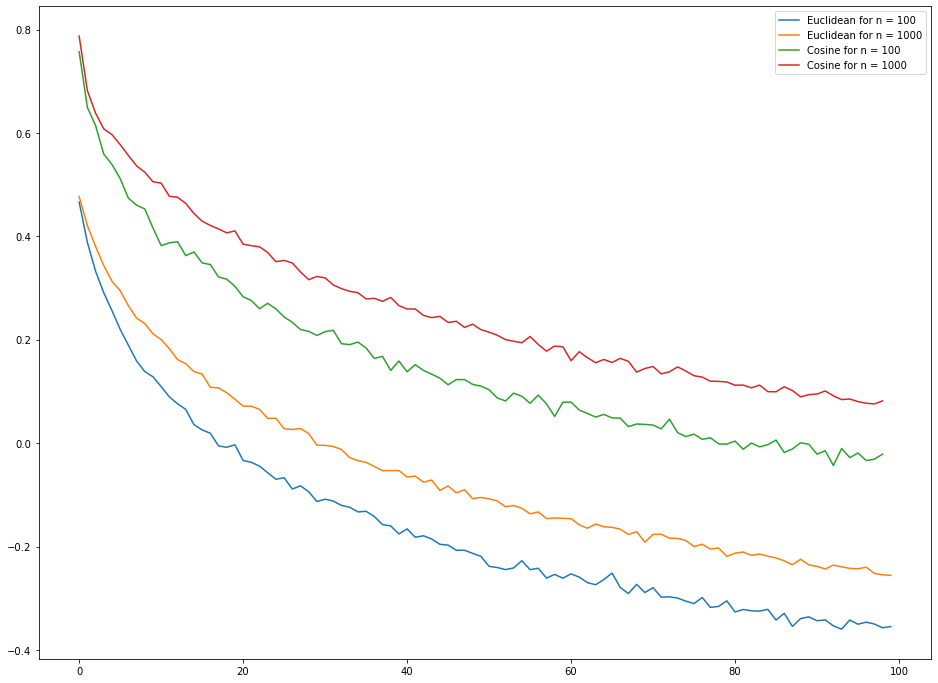
\includegraphics[width=18cm, keepaspectratio]{CurseOfDimensionality}
\end{center}

c)\\

Note that $k=1$ is a special case. Because the euclidian distance between two points can be though of as subtracting norms of two points. However, cosine similary between two points in 1-dimension is always 1 and hence $d_{cos}$ is $0$ for all possible combinations. Hence, $r(k)$ is not defined for $k = 1$.\\

The following holds for $k >= 2$:\\

\textbf{Case 1:} Predictions \& Observations within the same distance type:\\
I predicted that for a particular distance type, the spread of points is more when the dimensions are more. This increases the average of distance between points and probably the maximum.  Thus the value of $r(k)$ decreases as $k$ increases for a particular dataset size.
Again, as the number of data points increase the average distance decreases, thus increasing $r(k)$ for a particular value of $k$.
The above predictions imply $r(k)$ decreases as $k$ increases for a particualr $n$ and $r(k)$ and $r(k)$ increases as $n$ increases for a particular $k$.

The predictions are very much inline with the above plot.\\

\textbf{Case 2:} Predictions \& Observations across distance type:\\
It is hard to predict this comparison as is it is a difficult mathematical problem to compare euclidian distance vs cosine distance for random data with small magnitude. However, one can notice that for dimensions at least, for points with coordinates between $0$ \& $1$,  the maximum possible value for $r(k)_{max} = \log_{10}\left(2\right)$ is more likely to occur than that for euclidian distance,  because euclidian distance depends more on how far the points are located where as $d_{cos}$ depends more on orientation. Hence, we can plausibly say that $d_{cos} > d_{euc}$ at least for small dimensions.\\

This prediction is also inline with the observation in the above plot.
\end{solution}

\begin{problem}
Expectation-Maximization (EM) algorithm. Let $X$ be a random variable distributed according to
$$
p(x)=\alpha q\left(x \mid \lambda_{1}\right)+(1-\alpha) q\left(x \mid \lambda_{0}\right)
$$
where $\alpha \in(0,1),$ Let $q(x \mid \lambda)=\frac{\lambda}{x^{\lambda+1}}$ on the input space $[1, \infty)$ be a Pareto distribution with $\lambda>0 .$ Let now $\mathcal{D}=\left\{x_{i}\right\}_{i=1}^{n}$ be a set of observations.\\
a) (10 points) Derive update rules of the EM algorithm to estimate $\alpha, \lambda_{0},$ and $\lambda_{1}$.\\
b) (20 points) Implement the learning algorithm from part a and evaluate it on 100 simulated datasets with $n$ no less than $100 .$ Each dataset should be generated according to a distribution with fixed parameters. To assess the quality of your estimates, visualize the distribution of absolute differences between estimated and true parameters using box plots and compute the mean absolute difference. Discuss your experiments, discuss steps and calls you needed to make, and report on the quality of your algorithm.
\end{problem}

\begin{solution}
\\
\textbf{a)}
\\
Let, $w_k$ is the generic weight. Here, $w_1 = \alpha$ and $w_2 = 1 - \alpha$.\\
Similarly, let $\theta_k$ be the generic prameter for Pareto pdf. Here, $\theta_1 = \lambda_1$ and $\theta_2 = \lambda_0$.\\
The constraint is $\sum_{j=1}^{2}w_j = 1$.\\
We have two classes and hence after including the latent variables, the expected log likelihood takes the form,

$$
\mathbb{E}\left[\log p(\mathcal{D}, \boldsymbol{Y} \mid \theta) \mid \mathcal{D}, \theta\right]=\sum_{i=1}^{n} \sum_{j=1}^{2} \log \left(w_{j} p\left(x_{i} \mid \theta_{j}\right)\right) p_{Y_{i}}\left(j \mid x_{i}, \theta\right)
$$
To get $w_k$, consider the dependent terms.\\
Hence, the Lagrange function is,
$$
L_1(\boldsymbol{w}, \alpha) = \sum_{j=1}^{2} \log w_{j} \sum_{i=1}^{n} p_{Y_{i}}\left(j \mid x_{i}, \theta\right)+\alpha\left(\sum_{j=1}^{2} w_{j}-1\right)
$$
where $\alpha \neq 0$ is the Lagrange multiplier.
Then, by setting
$$
\begin{aligned}
\frac{\partial}{\partial w_{k}} L_1(\boldsymbol{w}, \alpha) &=0 \quad \forall \,k \in \mathcal{Y} \\
\frac{\partial}{\partial \alpha} L_2(\boldsymbol{w}, \alpha) &=0\\
\end{aligned}
$$
\\
Solving this and using the constraint, we get, $w_{k}=-\frac{\sum_{i=1}^{n} p_{Y_{i}}\left(k \mid x_{i}, \theta\right)}{\alpha}$ and $\alpha=-n$. Thus,
$$
\boxed{w_{k}=\frac{1}{n} \sum_{i=1}^{n} p_{Y_{i}}\left(k \mid x_{i}, \theta\right)}
$$
To get $\theta_k$, consider the dependent terms.\\
The pdf of Pareto distribution is, $p\left(x \mid \theta_{j}\right)$ with a parameter $\theta_{j};$ i.e., $p\left(x \mid \theta_{j}\right)=$ $\theta_{j} x^{-\theta_{j} - 1},$ where $\theta_{j}>0$. Hence, the Lagrange function is,
$$
L_2(\boldsymbol{w}, \alpha) = \sum_{j=1}^{2} \log p\left(x_{i} \mid \theta_{j}\right) \sum_{i=1}^{n} p_{Y_{i}}\left(j \mid x_{i}, \theta\right)
$$
for each $k \in \mathcal{Y}$, the set of latent variables. Substituting the pdf and differentiating w.r.t. $\theta_k$, we get,
$$
\frac{\partial}{\partial \theta_k}\left(\sum_{i=1}^{n} p_{Y_{i}}\left(k \mid x_{i}, \theta\right) \cdot\log(\theta_k)-(\theta_k+1)\cdot\sum_{i=1}^{n}p_{Y_{i}}\left(k \mid x_{i}, \theta\right) \cdot \log(x_i)\right)=0
$$
Solving this, we get,
$$
\boxed{\theta_{k}=\frac{\sum_{i=1}^{n}p_{Y_{i}}\left(k \mid x_{i}, \theta\right)}{\sum_{i=1}^{n} p_{Y_{i}}\left(k \mid x_{i}, \theta\right) \cdot \log(x_{i})}}
$$
Using Baye's Theorem we know that,
$$
p_{Y_{i}}\left(k \mid x_{i}, \theta\right)=\frac{w_{k} p\left(x_{i} \mid \theta_{k}\right)}{\sum_{j=1}^{2} w_{j} p\left(x_{i} \mid \theta_{j}\right)}
$$



This is an iterative algorithm.\\\\\\
\textbf{b)}\\\\
For code, please refer to \textbf{EMPareto.ipynb}\\\\
\textbf{Plot}\\
\begin{center}
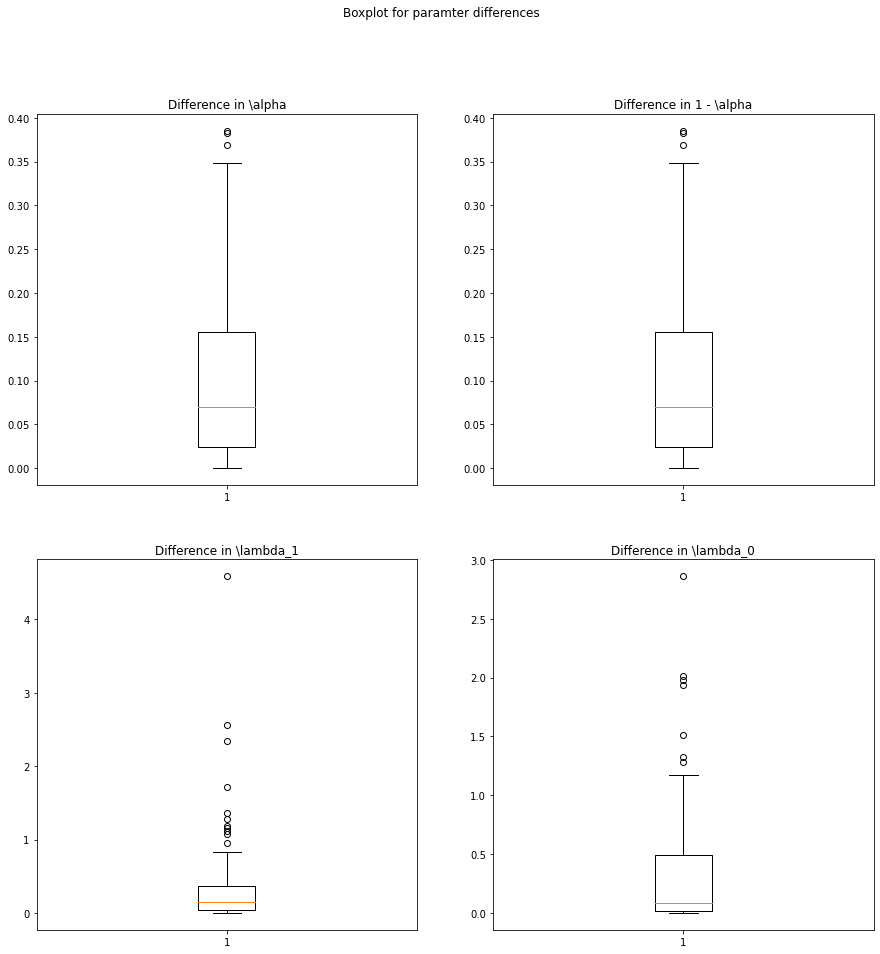
\includegraphics[width=18cm, keepaspectratio]{EMPareto}
\end{center}

I have derived the update rules as shown above. My dataset size is of $1000$ and I carry the experiment of running EM algorithm $100$ times. I generated the values for weights and parameters from a random uniform distribution between $0 \,\&\, 1$ and $0.01 \,\&\, 3$ respectively. In the softem algorithm, also I randomly choose the values for weights and paramaters from the same ranges. With a prior knowledge that the solution will necessarily converge, I have carried out the experiement till the point the parameters aren't updated until a difference less than $0.0001$ and found that it runs fairly quicker. I have computed the values for mean differences in weights and parameters and here are the values like:

\begin{lstlisting}
Mean absolute difference (\alpha) = 0.10525395212126394
Mean absolute difference (1 - \alpha) = 0.10525395212126394
Mean absolute difference (\lambda_1) = 0.366816910982778
Mean absolute difference (\lambda_0) = 0.33752129248324614
\end{lstlisting}

It is expected that mean absolute difference between two weights should be same because we have a constraint that both sum to $1$ and it implies that increase in one weight will reflect decrease in the other weight. It can be clearly seen from the first two values above. The mean absolute difference in parameters is 0.37, 0.34 which although seems relatively high it is not that bad because there are some outliers and hence mean is not a good central tendency measure here. Hence we can compare medians from the boxplots. The medians are almost close to zero showing that the parameters are estimated accurately at least 50 \% of the times.

\end{solution}

\end{document}
